\documentclass{article}
\usepackage[utf8]{inputenc}
\usepackage[frenchb]{babel}
\usepackage[T1]{fontenc}
\usepackage{graphicx}

\setlength{\oddsidemargin}{0pt} % Marge gauche sur pages impaires
\setlength{\evensidemargin}{9pt} % Marge gauche sur pages paires
\setlength{\marginparwidth}{54pt} % Largeur de note dans la marge
\setlength{\textwidth}{481pt} % Largeur de la zone de texte (17cm)
\setlength{\voffset}{-18pt} % Bon pour DOS
\setlength{\marginparsep}{7pt} % Séparation de la marge
\setlength{\topmargin}{0pt} % Pas de marge en haut
\setlength{\headheight}{13pt} % Haut de page
\setlength{\headsep}{10pt} % Entre le haut de page et le texte
\setlength{\footskip}{27pt} % Bas de page + séparation
\setlength{\textheight}{708pt} % Hauteur de la zone de texte (25cm)

\title{Rapport de Réseaux et Télécoms \\ Séance de TP 3}
\author{Florian Delavernhe et Thomas Minier \\ groupe 601A}
\date{Jeudi 12 Février 2014}

\begin{document}

\maketitle
\vspace{5cm}
\tableofcontents
\newpage

\section{Câblage et configuration des réseaux locaux}

Dans la première partie de ce TP, nous devons à l'aide du logiciel Marionnet câbler deux réseaux locaux.

\subsection{1er sous-réseau LAN1}
Le premier réseau comporte trois machines : \textbf{m1}, \textbf{m2} et \textbf{m3} reliées à un hub \textbf{h1} avec comme adresse 192.168.1.0/24. Grâce au netmask, on sait donc que c'est une adresse de classe C, l'adresse d'une machine reliée à ce réseau dépend donc du dernier octet.
Les adresses sont réparties comme suit :
\begin{verbatim}
m1 : 192.168.1.1
m2 : 192.168.1.2
\end{verbatim}

Nous utilisons la commande \textbf{ifconfig} pour attribuer les adresses :
\begin{verbatim}
ifconfig eth0 192.168.1.1/24 (exemple pour m1)
\end{verbatim}

Quant à \textbf{m3}, celle ci aura le rôle de passerelle, on lui attribut donc la dernier valeur possible, pour le réseau, en adresse à eth0. C'est a dire la plus grande valeur sur 8 bits moins 1 (car utilisé pour le broadcast) :
\begin{verbatim}
m3: 192.168.1.254	
\end{verbatim}

\subsection{2ème sous-réseau LAN2}

Pour le second réseau, nous câblons avec un hub \textbf{h2} deux machines : \textbf{m3} et \textbf{m4}. L'adresse du réseau est 10.10.0.0/16, de classe B donc les 2 derniers octets représentent les machines du réseau. Les adresses sont réparties ainsi (en eth0) :
\begin{verbatim}
m4 : 10.10.0.4
\end{verbatim}

L'adresse de \textbf{m3} pour ce réseau est encore une fois la dernière possible, donc la plus grande valeur possible pour les deux octets moins un pour le dernier octet, d'où (en eth1):
\begin{verbatim}
m4 : 10.10.255.254
\end{verbatim}

\section{Configuration du réseau étendu}

\subsection{Création d'un réseau LAN 1 + 2}

Nous allons maintenant relier les deux réseaux, et pour cela nous activons la fonctionnalité routage de \textbf{m3}, la passerelle, à l'aide de la commande suivante :
\begin{verbatim}
echo 1 >/proc/sys/ret/ipv4/ip_forward
\end{verbatim}

Nous modifions les tables de routage des machines de LAN1, pour pouvoir communiquer avec les machines de LAN2 et réciproquement afin de créer un réseau LAN1+2 contenant les deux sous-réseaux. Nous utilisons les commande suivantes :
\begin{verbatim}
route add -net 10.10.0.0/16 gw 192.168.1.254    (Pour une machine de LAN1 a LAN2)	
route add -net 192.168.0.0/24 gw 10.10.255.254/16   (Pour une machine de LAN2 a LAN1)
\end{verbatim}

Où 10.10.0.0 représente l'adresse avec laquelle nous souhaitons établir la route, /16 son netmask, et 192.168.1.254 l'adresse de la passerelle dans notre réseau local qui nous permet de communiquer avec l'adresse que l'on souhaite rejoindre. \newpage

\subsection{Est-il utile de modifier la table de routage de m3 ?}

Il est inutile de modifier la table de routage de \textbf{m3}, la passerelle, car \textbf{m3} est déjà relié à \textbf{h1} par eth0 et \textbf{h2} par eth1. De plus, il existe déjà une route entre eth0 et eth1, car les deux interfaces sont situées sur la même machine .

Après test de la commande ping entre \textbf{m1} et \textbf{m4}, on obtient un résultat positif, donc la route est bien établie.

\subsection{Utilisation d'une passerelle par défaut}

Nous supprimons l’ensemble des routes créées précédemment à l'aide de la commande \textbf{route del}. Ensuite nous utilisons la commande suivante :
\begin{verbatim}
route add default gw 192.168.1.254  (pour m1 et m2)
route add default gw 10.10.255.254  (pour m4)
\end{verbatim}

Ces commandes nous permettent de créer le même réseau que ce que nous avons fais précédemment : l'option \textbf{default} permet d'indiquer à la machine qu'à chaque fois qu'elle cherchera une autre machine, elle doit passer par \textbf{m3}. Or, \textbf{m3} étant une passerelle reliée à LAN1 et LAN2, la machine peut donc communiquer avec les deux réseaux. On a donc recréé le réseau LAN1+2.
\begin{figure}[h]
\centering
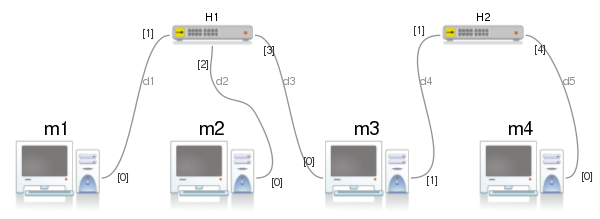
\includegraphics[scale=0.5]{capture-1-passerelle.png}
\caption{Réseau LAN 1 + 2}
\end{figure}

Cependant, si l'on ajoute un autre réseau LAN3, avec laquelle on souhaite relier LAN1+2 à l'aide d'une autre passerelle que \textbf{m3} dans LAN1, on  doit reconfigurer chaque élément de LAN1 sans utiliser \textbf{default}. En effet, s'il y a plusieurs passerelle dans le même réseau, alors on ne peut plus utiliser cette option, sinon les machines de ce réseau ne pourrons passer que par une seul passerelle en ignorant l'autre et une partie du réseau deviendra inaccessible. ce cas de figure est illustré par le schéma suivant : 
\begin{figure}[h]
\centering
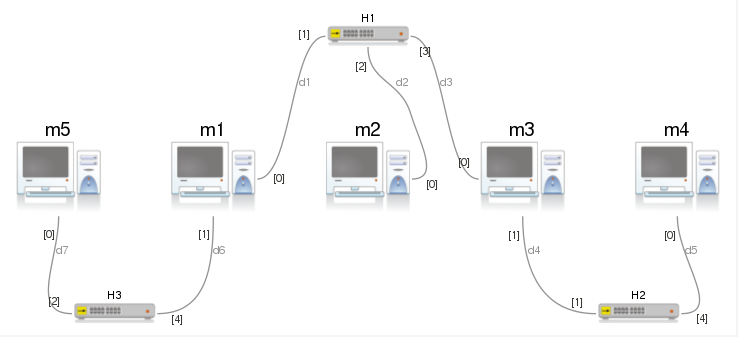
\includegraphics[scale=0.5]{capture-deux-passerelles.png}
\caption{Cas d'un réseau sans passerelle par défaut}
\end{figure} \newpage

\section{Le rôle de ICMP dans le routage IP : un cas de figure}

Nous commençons par éteindre toutes les machines afin de pouvoir recommencer sans aucune route ou configuration.

Nous utilisons ensuite à partir de \textbf{m1} :
\begin{verbatim}
ping 10.10.0.4 
\end{verbatim}

Pour essayer de ping \textbf{m4} a partir de \textbf{m1}, et obtenons un message d'erreur qui nous indique que \textbf{m1} n'existe pas dans le réseau, donc nous avons bien tout recommencer. \\

Ensuite nous utilisons sur \textbf{m1}:
\begin{verbatim}
ifconfig eth0 192.168.0.1
\end{verbatim}

Afin de configurer l'IP de \textbf{m1}. Puis nous ressayons de ping \textbf{m4}. Résultat : il n'y a pas de réponse et donc 100\% des paquets perdus. En effet, \textbf{m1} ping le réseau de \textbf{h1} à la recherche de l'adresse de \textbf{m4} mais il n'y aucune machine relié à \textbf{h1}. \\

Nous configurons maintenant sur \textbf{m1} l'ancienne adresse de \textbf{m3} en tant que passerelle par défaut. Nous réutilisons donc la commande suivante : 
\begin{verbatim}
route add default gw 192.168.1.254
\end{verbatim}

Nous envoyons un ping de \textbf{m1} à \textbf{m4} et on laisse boucler. Nous observons le résultat suivant : 
\begin{verbatim}
arp who_has 192.168.1.254 tell 192.168.1.1
\end{verbatim}

Ce message nous montre que suite à la configuration de \textbf{m3} comme passerelle par défaut, \textbf{m1} cherche a envoyer son message à la passerelle (donc à l'ancienne adresse de \textbf{m3}) pour que celui ci l'envoie a l'adresse de \textbf{m4}. Or \textbf{m3} n'a toujours pas d'adresse attribuée, il n'y a donc pas d'adresse 192.168.1.254 sur le réseau. Le hub continue donc d'interroger toutes les machines branchées pour savoir qui possède l'adresse 192.168.1.254 afin d'envoyer le message de \textbf{m1}. C'est un protocole \textbf{ARP}.

Ensuite, nous configurons les interfaces eth0 et eth1 sur \textbf{m3}, a l'aide de commande vues précédemment.
Nous observons un changement suite à la configuration de eth0 :
\begin{verbatim}
IP 192.168.1.1 > 10.10.0.4 ICMP echo request … 
\end{verbatim}

Ce message nous indique que le hub \textbf{h1} a enfin trouver la passerelle d'adresse 192.168.1.254, puisque nous avons relié eth0 de \textbf{m3} à \textbf{h1} et on lui a attribué cette adresse, celui-ci envoie donc maintenant le ping de \textbf{m1} vers \textbf{m4} vers l'ensemble des réseaux auxquels elle est connectée, c'est à dire LAN1.

Suite à la configuration de eth1 de \textbf{m3}, il ne se passe rien de plus, eth0 et eth1 de \textbf{m3} ne sont pas encore reliées car \textbf{m3} n'est toujours pas une passerelle.

Nous activons ensuite le routage de m3. Nous observons des changements immédiats sur l'affichage du termina espion de \textbf{m4} :
\begin{verbatim}
arp who_has 10.10.0.4 tell 10.10.1.254
\end{verbatim}

Ce message nous indique que le ping de \textbf{m1} reçu de la passerelle \textbf{m3}, a été envoyé par \textbf{m3} sur le hub \textbf{h2} pour rechercher l'adresse 10.10.0.4, mais comme nous n'avons toujours pas configurer \textbf{m4}, cette adresse n'est toujours pas attribuée, et donc le hub continue de chercher qui possède cette adresse.

Quant à LAN1, le terminal espion sur \textbf{m2} nous indique, en l'absence de réponse de la passerelle, que le destinataire est inaccessible. \\

Nous configurons ensuite l'eth0 de \textbf{m4}, celui ci est donc maintenant relié au réseau \textbf{h2}, donc le ping lui est transmis car il est possède l'adresse que le hub recherche, et donc \textbf{m1} n'affiche plus que le destinataire est inaccessible.
	Cependant, on observe que, dans les deux sous-réseaux, on attend toujours une réponse au ping. En effet, \textbf{m4} ne peut pas transmettre sa réponse, il l'envoie sur le réseau via \textbf{h2} mais aucune machine ne possède cette adresse.

Nous configurons donc \textbf{m3} comme passerelle par défaut pour \textbf{m4}, cette dernière envoie donc son message à \textbf{m3} qui transmet ensuite la réponse à \textbf{m1}. Il y a donc bien un envoi et réception du message, et envoie et réception de son accusé, tout fonctionne normalement.

\end{document}
